\chapter{The Gaussian Chain Solved Exactly}\label{ch:gaussian}

This chapter answers RQ1. We take the simplest data distribution with
genuine internal structure --- the stationary Gaussian AR(1) chain of
Section~\ref{sec:ar1} --- corrupt every frame with the OU channel of
Section~\ref{sec:ou}, and compute the joint score \emph{exactly}, twice: once
by linear algebra, once by Bayesian inference. The two routes must agree, and
verifying that they do (to machine precision) is the first audit of the
computational companion. We then characterise the complete lifecycle of the
score's coupling structure --- the posterior precision matrix --- from the
sparse Markov regime at $t \to 0$ to the isotropic regime at $t \to \infty$,
including a corrected small-$t$ \emph{band-fill law} and exact closed forms
for the bulk of a long chain. Throughout, longer algebraic passages are
isolated in toolboxes, and every boxed formula is covered by a named check of
the numerical audit (Appendix~\ref{app:repro}).

\section{The model, and the object of study}\label{sec:g-model}

\paragraph{Data.} A single data point is a trajectory
$a = (a_0, \dots, a_{K-1}) \in \R^K$ of the stationary AR(1) chain
\eqref{eq:ar1},
\begin{equation}
  a_{k+1} = \alpha\, a_k + \eta_k,
  \qquad \eta_k \sim \Nd(0, \sigma_\eta^2)\ \text{i.i.d.},
  \qquad a_0 \sim \Nd(0, 1),
  \label{eq:g-ar1}
\end{equation}
with $|\alpha| < 1$ and the \emph{stationary normalisation}
$\sigma_\eta^2 = 1 - \alpha^2$, which makes the marginal variance of every
frame equal to $1$ (Toolbox~\ref{tb:ar1}). One should think of $k$ as an
\emph{internal} (frame) time --- the index along the video --- to be kept
sharply distinct from the diffusion time $t$.

\paragraph{Corruption.} Each frame passes independently through the OU
channel \eqref{eq:ou-channel} for a time $t$:
\begin{equation}
  x_k \;=\; e^{-t} a_k + \sqrt{\Deltat}\;\xi_k,
  \qquad \xi_k \sim \Nd(0,1)\ \text{i.i.d.},
  \qquad \Deltat = 1 - e^{-2t}.
  \label{eq:g-channel}
\end{equation}

\paragraph{Object of study.} The \emph{joint score} of the noisy sequence,
\begin{equation}
  \score(x, t) \;=\; \nabla_x \log P_t(x) \;\in\; \R^K,
  \qquad
  P_t(x) = \int_{\R^K} P_0(a) \prod_{k=0}^{K-1}
    \Nd\big(x_k;\, e^{-t}a_k,\, \Deltat\big)\, \dd a .
  \label{eq:g-object}
\end{equation}
We stress \emph{joint}: the gradient is taken with respect to all $K$ noisy
frames simultaneously, under the law of the whole noisy trajectory. The
per-frame \emph{marginal} score $\partial_{x_k} \log p_t(x_k)$ is a
different, strictly less informative object --- for this model it is
actually degenerate, as Section~\ref{sec:g-K2} shows --- and conflating the
two was an instructive early error of this project, corrected in
supervision: a sequence is \emph{one} sample from a joint law, not $K$
samples from marginal laws. Only the joint score drives the reverse dynamics
of the sequence as a whole, by Anderson's theorem
(Section~\ref{sec:reversal}) applied in $\R^K$.

\section{The clean joint law: dense covariance, sparse precision}
\label{sec:g-clean}

The chain factorisation \eqref{eq:chain-factorisation} gives the clean joint
density
\begin{equation}
  P_0(a)
  = \Nd(a_0; 0, 1) \prod_{k=0}^{K-2}
    \Nd\big(a_{k+1};\, \alpha a_k,\, \sigma_\eta^2\big)
  = \Nd(a;\, 0,\, \Sigz),
  \label{eq:g-P0}
\end{equation}
a centred Gaussian whose two natural parametrisations --- covariance and
precision --- encode the chain's structure in opposite ways.

\begin{proposition}[Stationary covariance]\label{prop:g-Sigma0}
$(\Sigz)_{ij} = \alpha^{|i-j|}$ for all $i, j$: a dense, symmetric Toeplitz
matrix with geometrically decaying off-diagonals.
\end{proposition}

This was derived in Toolbox~\ref{tb:ar1} (unrolling the recursion);
stationarity is
what makes the entries depend on $i - j$ only, i.e.\ what makes $\Sigz$
Toeplitz.

\begin{proposition}[Tridiagonal precision]\label{prop:g-Q0}
$\Qz := \Sigz^{-1}$ is exactly tridiagonal:
\begin{equation}
  (\Qz)_{kk} =
  \begin{cases}
    \dfrac{1}{\sigma_\eta^2}, & k \in \{0, K-1\},\\[8pt]
    \dfrac{1+\alpha^2}{\sigma_\eta^2}, & 0 < k < K-1,
  \end{cases}
  \qquad
  (\Qz)_{k, k\pm 1} = -\frac{\alpha}{\sigma_\eta^2},
  \label{eq:g-Q0}
\end{equation}
and every entry at distance $\geq 2$ vanishes identically.
\end{proposition}

\begin{toolbox}{Deriving the tridiagonal precision from the log-density}
For a centred Gaussian, the precision is the Hessian of the negative
log-density. From \eqref{eq:g-P0},
\begin{equation*}
  -2 \log P_0(a)
  = \frac{a_0^2}{\sigma_0^2}
  + \sum_{k=0}^{K-2} \frac{(a_{k+1} - \alpha a_k)^2}{\sigma_\eta^2}
  + \text{const},
  \qquad \sigma_0^2 = 1 .
\end{equation*}
Read off the quadratic form term by term.
\emph{Off-diagonals:} the only term coupling $a_k$ and $a_{k+1}$ is the
transition $(a_{k+1} - \alpha a_k)^2 / \sigma_\eta^2$, whose cross
coefficient is $-2\alpha/\sigma_\eta^2$, i.e.\ a precision entry
$-\alpha/\sigma_\eta^2$; \emph{no term couples variables at distance
$\geq 2$}, so those precision entries are exactly zero.
\emph{Interior diagonal:} $a_k$ appears in its left transition with
coefficient $1/\sigma_\eta^2$ and in its right transition with coefficient
$\alpha^2/\sigma_\eta^2$; sum: $(1+\alpha^2)/\sigma_\eta^2$.
\emph{Left boundary:} prior term $1/\sigma_0^2 = (1-\alpha^2)/\sigma_\eta^2$
plus right transition $\alpha^2/\sigma_\eta^2$, summing to
$1/\sigma_\eta^2$; the right boundary is symmetric (left transition only).
\hfill$\square$
\end{toolbox}

\begin{remark}[Tridiagonality is Markovianity, not Gaussianity]
\label{rmk:g-markov-sparsity}
A zero in the precision matrix is a conditional independence given all other
variables (the Hammersley--Clifford fingerprint, formalised in
Section~\ref{sec:mrf}). The derivation above used Gaussianity only to
identify the precision with the Hessian of $-\log P_0$; the \emph{support}
of that Hessian --- nearest neighbours only --- comes from the chain
factorisation alone. Any Markov chain with smooth transitions has this
sparsity pattern in $\nabla^2(-\log P_0)$; the Gaussian case just makes the
entries constants. This tridiagonal $\Qz$ is the only sparse object in the
whole story, and every structural result below traces back to it.
\end{remark}

The pair (Propositions~\ref{prop:g-Sigma0}, \ref{prop:g-Q0}) is worth
contemplating: the \emph{covariance} is dense --- every frame correlates
with every other, at geometrically decaying strength --- while the
\emph{precision} is tridiagonal. Correlation is global; conditional
dependence is local. The score, we now show, is governed by the second
object.

\section{The noisy joint law and the score, two ways}\label{sec:g-score}

\subsection{Route one: linear algebra}

\begin{proposition}[Noised law]\label{prop:g-Sigt}
$P_t(x) = \Nd(x;\, 0,\, \Sigt)$ with
\begin{equation}
  \boxed{\;\Sigt \;=\; e^{-2t}\, \Sigz \;+\; \Deltat\, I_K\;}
  \label{eq:g-Sigt}
\end{equation}
\end{proposition}
This is \eqref{eq:ou-cov-map}: the linear channel contracts the signal
covariance and adds white noise; Gaussianity is preserved because an affine
map plus independent Gaussian noise of a Gaussian is Gaussian. Note the
diagonal: $e^{-2t} + \Deltat = 1$ at every $t$ (variance preservation);
only the \emph{off-diagonal} entries, $\alpha^{|i-j|} e^{-2t}$, feel the
diffusion time --- the noise of different frames is independent, so only
the signal correlates.

Since $\log P_t(x) = -\tfrac{1}{2} x^\T \Sigt^{-1} x + \text{const}$,
\begin{equation}
  \boxed{\;\score(x, t) \;=\; -\,\Sigt^{-1} x \;=\; -\,\Qt\, x,
  \qquad \Qt := \Sigt^{-1}.\;}
  \label{eq:g-score-matrix}
\end{equation}
The joint score is \emph{linear} in $x$ --- the hallmark of Gaussianity ---
and its entire structure is the noisy precision matrix $\Qt$: every question
about the score (which frames talk to which, how strongly, at which $t$) is
a question about a matrix. Sections~\ref{sec:g-lifecycle} and
\ref{sec:g-bulk} answer those questions completely.

\subsection{Route two: Bayesian inference}

The score--posterior identity \eqref{eq:tweedie-joint} expresses the same
score through the posterior mean of the clean chain:
\begin{equation}
  \score_k(x, t)
  = \frac{e^{-t}\, \E[a_k \,|\, x] - x_k}{\Deltat} .
  \label{eq:g-tweedie}
\end{equation}
The posterior is itself Gaussian, with parameters worth recording once and
using forever:

\begin{proposition}[Posterior of the clean chain]\label{prop:g-posterior}
$P(a \,|\, x) = \Nd(a;\, m,\, J^{-1})$ with
\begin{equation}
  \boxed{\;
  J \;=\; \frac{e^{-2t}}{\Deltat}\, I \;+\; \Qz ,
  \qquad
  J\, m \;=\; h := \frac{e^{-t}}{\Deltat}\, x .
  \;}
  \label{eq:g-posterior}
\end{equation}
\end{proposition}

\begin{toolbox}{Posterior precision and field, by completing the square}
Bayes' rule with the likelihood \eqref{eq:g-channel}:
\begin{align*}
  -2 \log P(a | x)
  &= a^\T \Qz\, a
  + \sum_{k} \frac{(x_k - e^{-t} a_k)^2}{\Deltat}
  + \text{const} \\
  &= a^\T \Big( \Qz + \tfrac{e^{-2t}}{\Deltat} I \Big) a
  - 2\, \tfrac{e^{-t}}{\Deltat}\, x^\T a
  + \text{const}.
\end{align*}
Matching against the generic Gaussian form
$a^\T J a - 2 h^\T a$ gives \eqref{eq:g-posterior} directly. Two structural
observations. (i) The likelihood is \emph{diagonal} in $a$: observing each
frame through its own channel adds $e^{-2t}/\Deltat$ --- the
signal-to-noise ratio of the channel, divergent as $1/2t$ at small $t$,
vanishing at large $t$ --- to every diagonal entry of the prior precision,
and touches nothing else. (ii) Consequently $J$ is \emph{tridiagonal at
every $t$}: the posterior of the clean chain remains a nearest-neighbour
MRF; what fills up with $t$ is the precision of the \emph{noisy} law,
$\Qt$, not of the posterior. Keeping $J$ (tridiagonal, posterior) and
$\Qt$ (dense, noisy marginal) distinct prevents much confusion.
\hfill$\square$
\end{toolbox}

Substituting the linear posterior mean $m = J^{-1} h$ into
\eqref{eq:g-tweedie} must return $-\Qt x$ identically. It does --- one can
verify the operator identity
$\frac{1}{\Deltat}\big( e^{-2t} J^{-1} \tfrac{1}{\Deltat} - I \big) = -\Qt$
directly from \eqref{eq:g-Sigt} and \eqref{eq:g-posterior} by the
Woodbury identity --- and the computational companion checks the two routes
agree to $2.7 \times 10^{-15}$ across sweeps of $(K, \alpha, t)$. The
agreement is a genuine end-to-end audit: a $K \times K$ inversion against a
Bayesian smoothing computation, built from different formulas.

\subsection{$K = 2$: the smallest example, fully explicit}\label{sec:g-K2}

Everything above, written where nothing can hide. For $K = 2$,
\begin{equation}
  \Sigt = \begin{pmatrix} 1 & r \\ r & 1 \end{pmatrix},
  \qquad \boxed{\; r = \alpha\, e^{-2t} \;}
  \qquad\Longrightarrow\qquad
  \Qt = \frac{1}{1 - r^2}
  \begin{pmatrix} 1 & -r \\ -r & 1 \end{pmatrix},
  \label{eq:g-K2}
\end{equation}
\begin{equation}
  \score_0(x, t) = -\,\frac{x_0 - r\, x_1}{1 - r^2},
  \qquad
  \score_1(x, t) = -\,\frac{x_1 - r\, x_0}{1 - r^2}.
  \label{eq:g-K2-score}
\end{equation}
Contrast with the marginal score: each $x_k$ is $\Nd(0,1)$ at every $t$
(variance preservation), so $\partial_{x_k} \log p_t(x_k) = -x_k$,
independent of $t$ and of the other frame --- the marginal score of this
model \emph{carries no information about the dynamics at all}. The joint
score \eqref{eq:g-K2-score} instead contains the cross term $-r x_1$: the
denoiser of frame $0$ borrows evidence from frame $1$ with weight
$r = \alpha e^{-2t}$ --- the whole coupling lifecycle in miniature, equal to
$\alpha$ at $t = 0$, decaying exponentially, gone at $t \to \infty$.

\section{The spectral form and the lifecycle of the precision matrix}
\label{sec:g-lifecycle}

How does $\Qt$ interpolate between its two known endpoints --- the
tridiagonal $\Qz$ at $t = 0$ and the identity at $t = \infty$? This section
proceeds in the order the question deserves: first the two pieces of linear
algebra the analysis rests on, then the \emph{spectral form} of $\Qt$ ---
the master representation from which everything else follows --- and then
the study itself: when tridiagonality is lost, how fast, and how much, as
diffusion time runs.

\subsection{The linear algebra we need}\label{sec:g-linalg}

\begin{theorem}[Spectral theorem for symmetric matrices]\label{thm:g-spectral}
Every symmetric $A \in \R^{K \times K}$ admits an orthonormal eigenbasis:
there exist an orthogonal matrix $U$ (columns $u_1, \dots, u_K$,
$U^\T U = I$) and real numbers $\omega_1, \dots, \omega_K$ with
\begin{equation}
  A \;=\; U \operatorname{diag}(\omega_i)\, U^\T
  \;=\; \sum_{i=1}^{K} \omega_i\, u_i u_i^\T .
  \label{eq:g-spectral-thm}
\end{equation}
\end{theorem}

Two consequences carry the whole section. \emph{First}, analytic operations
act on the eigenvalues alone: for any function $f$ defined on the spectrum,
$f(A) = U \operatorname{diag}(f(\omega_i))\, U^\T$; in particular
$A^{-1} = U \operatorname{diag}(1/\omega_i)\, U^\T$ whenever no eigenvalue
vanishes. \emph{Second}, affine images share the eigenbasis: for scalars
$c, d$,
\begin{equation}
  (c A + d I)\, u_i \;=\; (c\, \omega_i + d)\, u_i ,
  \label{eq:g-affine-eig}
\end{equation}
so $cA + dI$ has the \emph{same} eigenvectors as $A$, with eigenvalues moved
by the same affine map. Both facts are elementary; their power here comes
from the specific structure of our matrices. The clean covariance $\Sigz$
is symmetric Toeplitz --- constant along diagonals, because the chain is
stationary --- and the eigenvectors of large symmetric Toeplitz matrices
are asymptotically the Fourier modes of the sequence: stationary processes
are diagonalised by frequency \citep{brockwell1991time}. So the eigenbasis
$U$ we are about to fix for all diffusion times is, up to boundary effects,
the Fourier basis of the chain.

\subsection{The spectral form of $\Sigt$ and $\Qt$}

Now apply \eqref{eq:g-affine-eig} to the forward map
\eqref{eq:g-Sigt}, $\Sigt = e^{-2t} \Sigz + \Deltat I$, which is affine in
$\Sigz$ with $c = e^{-2t}$, $d = \Deltat$:

\begin{theorem}[Spectral form]\label{thm:g-three-forms}
Let $\Sigz = U \operatorname{diag}(\omega_i) U^\T$. Then for \emph{every}
$t \geq 0$,
\begin{equation}
  \boxed{\;
  \Sigt = U \operatorname{diag}\big( \lambda_i(t) \big) U^\T,
  \qquad
  \Qt = U \operatorname{diag}\!\Big( \frac{1}{\lambda_i(t)} \Big) U^\T,
  \qquad
  \lambda_i(t) = e^{-2t} \omega_i + \Deltat .
  \;}
  \label{eq:g-Qt-spec}
\end{equation}
\end{theorem}

The content of \eqref{eq:g-Qt-spec} is that diffusion never rotates the
problem: \emph{the eigenvectors of $\Sigt$ and $\Qt$ are those of $\Sigz$,
frozen for all $t$} --- only the eigenvalues flow, each along the same
affine path $\omega_i \mapsto e^{-2t}\omega_i + \Deltat$, all monotonically
towards $1$ (Figure~\ref{fig:g-spectral}). In the eigenbasis the denoising
problem is $K$ independent scalar problems at every diffusion time. Two
computational corollaries, recorded for later use: factoring $\Deltat$ out
of \eqref{eq:g-Sigt} gives the \emph{SNR form}
\begin{equation}
  \Qt = \tfrac{1}{\Deltat} \big( I + \gamma_t\, \Sigz \big)^{-1},
  \qquad \gamma_t := e^{-2t}/\Deltat ,
  \label{eq:g-Qt-snr}
\end{equation}
and multiplying \eqref{eq:g-Sigt} by $\Qz$ and inverting gives the
\emph{resolvent form}
\begin{equation}
  \Qt = e^{2t}\, \Qz \big( I + c_t \Qz \big)^{-1}
      = e^{2t} \sum_{m \geq 0} (-c_t)^m\, \Qz^{\,m+1},
  \qquad c_t := e^{2t} - 1 ,
  \label{eq:g-Qt-res}
\end{equation}
whose Neumann series converges for $\|c_t \Qz\| < 1$, i.e.\ at small $t$
--- exactly where we deploy it below.

\subsection{Losing tridiagonality: when, how, and how much}
\label{sec:g-tridiag-loss}

The spectral form seems to say that nothing ever changes structurally: the
same modes, drifting eigenvalues. The tension with the $t = 0$ picture ---
an exactly tridiagonal $\Qz$ --- dissolves once one remembers that
\emph{sparsity is a property of a matrix in a basis}. In the eigenbasis the
problem is diagonal at all times; in the \emph{frame} basis --- the
operationally meaningful one, since a score architecture reads frames, not
Fourier modes --- the zeros of $\Qz$ are a delicate cancellation, and
diffusion destroys it. The destruction is precisely quantifiable, and it
answers the three questions the supervision programme poses: \emph{when} is
tridiagonality lost, \emph{how} does it happen, and \emph{how much}
structure survives at each $t$.

\paragraph{When: immediately.} By \eqref{eq:g-Qt-spec} every entry of
$\Qt$ is an analytic function of $t$. The distance-$d$ entries, identically
zero at $t = 0$ for $d \geq 2$, become non-zero for every $t > 0$: the
Markov conditional-independence structure is not eroded gradually --- it is
lost \emph{instantly}, in the sense that no exact zero survives any positive
diffusion time.

\paragraph{How: one diagonal per order in $t$.} The loss is nevertheless
graded, and the resolvent form gives the exact rate at which each diagonal
switches on (Figure~\ref{fig:g-lifecycle}).

\begin{figure}[t]\centering
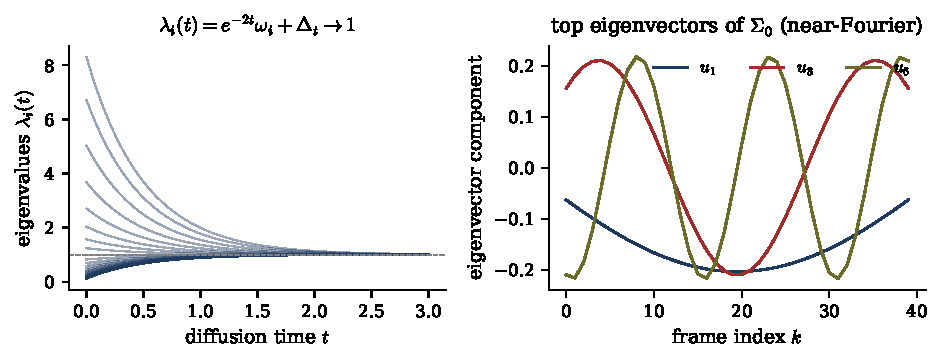
\includegraphics[width=\linewidth]{figures/fig_spectral.pdf}
\caption{\textbf{Spectral lifecycle.} Left: the eigenvalues of $\Sigt$ flow
as $\lambda_i(t) = e^{-2t}\omega_i + \Deltat$, all monotonically towards
$1$. Right: eigenvectors of $\Sigz$ --- shared by $\Sigt$ and $\Qt$ at
every $t$ by Theorem~\ref{thm:g-three-forms} --- are near-Fourier modes of
the chain.}
\label{fig:g-spectral}
\end{figure}

\begin{figure}[t]\centering
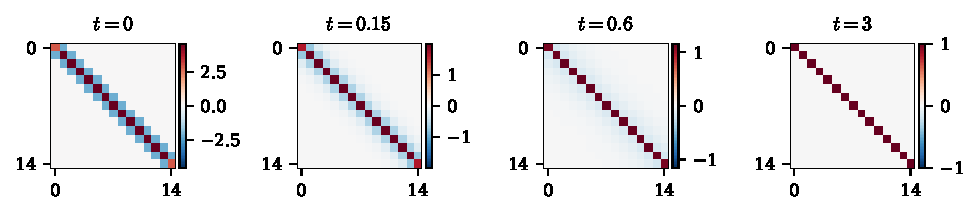
\includegraphics[width=\linewidth]{figures/fig_precision_lifecycle.pdf}
\caption{\textbf{Lifecycle of $\Qt$ in the frame basis} ($K = 15$,
$\alpha = 0.8$): exactly tridiagonal at $t = 0$ (Markov structure), the
band fills at intermediate $t$ (every frame couples to every other), and
the matrix collapses to the identity as $t \to \infty$ (isotropic noise
wins).}
\label{fig:g-lifecycle}
\end{figure}

\begin{theorem}[Band-fill leading order]\label{thm:g-bandfill}\label{sec:g-bandfill}
For small $t$ and frame distance $d \geq 1$,
\begin{equation}
  \boxed{\;
  (\Qt)_{i, i+d}
  \;=\; (-1)^{d-1}\, (2t)^{d-1}\, \big( \Qz^{\,d} \big)_{i, i+d}
  \;+\; O(t^{d}) .
  \;}
  \label{eq:g-bandfill}
\end{equation}
\end{theorem}

\begin{toolbox}{Band fill from the Neumann series}
In the resolvent form \eqref{eq:g-Qt-res}, substitute
$c_t = 2t + 2t^2 + O(t^3)$ and $e^{2t} = 1 + O(t)$:
\begin{equation*}
  \Qt = \big(1 + O(t)\big)
  \Big[ \Qz - c_t \Qz^2 + c_t^2 \Qz^3 - \cdots \Big].
\end{equation*}
$\Qz$ is tridiagonal, so $\Qz^{\,m}$ has bandwidth $m$: the entry at
distance $d$ receives its \emph{first} contribution from the single term
$m = d$ of the series, which carries the prefactor
$(-c_t)^{d-1} = (-1)^{d-1} (2t)^{d-1} (1 + O(t))$. Every later term is
$O(t^d)$. Each additional frame of coupling range costs one power of $t$:
the band fills \emph{outward, one diagonal per order}. \hfill$\square$
\end{toolbox}

\begin{remark}[Correction of an earlier formula]\label{rmk:g-correction}
An earlier working note of this project stated \eqref{eq:g-bandfill} with an
extraneous factor $1/(d-1)!$. The factor does not follow from the resolvent
expansion --- the leading distance-$d$ term is a \emph{single} Neumann term,
with no combinatorial sum behind it --- and the numerical audit rejects it:
the no-factorial coefficient matches the measured
$(\Qt)_{i,i+d}/t^{d-1}$ to better than $0.9\%$ for every $d \in \{1,\dots,5\}$
(at $\alpha = 0.9$, $K = 25$), while the factorial version fails by
$86\%$ at $d = 3$, $290\%$ at $d = 4$ and over $800\%$ at $d = 5$.
Instructively, the error had survived because empirical \emph{slope} fits
(exponent $d-1$ in $t$) are blind to constant prefactors; only auditing the
coefficient itself exposed it. Every prefactor in this thesis has since been
audited, not only every exponent.
\end{remark}

\begin{figure}[t]\centering
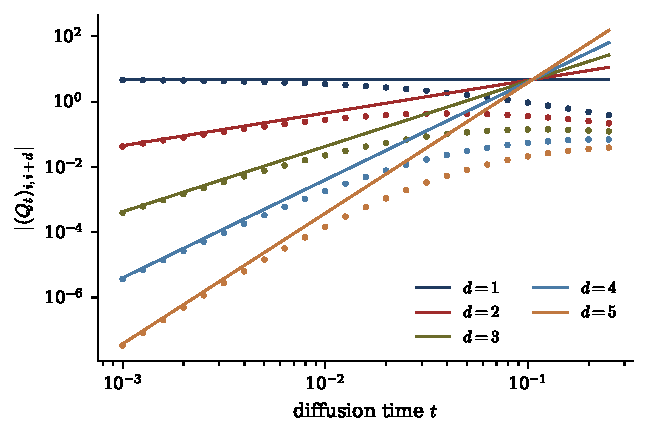
\includegraphics[width=0.78\linewidth]{figures/fig_band_fill.pdf}
\caption{\textbf{Band-fill law, log--log.} Measured $|(\Qt)_{i,i+d}|$ against
$t$ (dots) and the leading order \eqref{eq:g-bandfill} (solid lines --- no
fitted parameters). The slopes are $d - 1 = 0, \dots, 4$; agreement at small
$t$ is at the percent level for every $d$.}
\label{fig:g-bandfill}
\end{figure}

\paragraph{How much: the off-tridiagonal mass across diffusion time.}
The two regimes join into a single quantitative curve. Define the
off-tridiagonal Frobenius mass of $\Qt$ --- the norm of everything outside
the band that Markov structure would allow. At small $t$ the band-fill law
says each new diagonal contributes at its own power of $t$, so the mass
rises from zero, dominated by the $d = 2$ diagonal, linearly in $t$. At
large $t$, writing $\Sigt = I + e^{-2t}(\Sigz - I)$ and expanding the
inverse,
\begin{equation}
  \Qt = I - e^{-2t}(\Sigz - I) + e^{-4t}(\Sigz - I)^2 + O(e^{-6t}),
  \label{eq:g-larget}
\end{equation}
so $\| \Qt - I \|_F \simeq e^{-2t} \|\Sigz - I\|_F$: \emph{all} structure
--- off-tridiagonal and tridiagonal alike --- dies at the universal rate
$e^{-2t}$, and the score collapses onto the isotropic $-x$. In between, the
off-tridiagonal mass peaks (Figure~\ref{fig:g-tridiagloss}): the noisy
sequence is \emph{most} non-Markov at intermediate diffusion times, which
is precisely the regime where generative sampling spends its structurally
decisive steps. The full lifecycle, in one line: \emph{sparse} (tridiagonal,
Markov) at $t = 0$; densifying at rate $t^{d-1}$ per diagonal $d$;
maximally coupled at intermediate $t$; \emph{isotropic} at $t \to \infty$
at rate $e^{-2t}$.

\begin{figure}[t]\centering

\includegraphics[width=0.78\linewidth]{figures/fig_tridiag_loss.pdf}
\caption{\textbf{Structure lost and recovered, one curve each.}
$\|\Sigt - \Sigz\|_F$ (navy) grows monotonically as the covariance is driven
to the identity; the off-tridiagonal Frobenius mass of $\Qt$ (red) rises
from zero, peaks at intermediate $t$, and decays back to zero: the band
fills, then empties.}
\label{fig:g-tridiagloss}
\end{figure}

\section{The bulk of a long chain, in closed form}\label{sec:g-bulk}

For a long chain, the interior (``bulk'') is translation invariant and
everything can be solved exactly. By Proposition~\ref{prop:g-posterior} the
posterior precision in the bulk is the tridiagonal Toeplitz matrix with
\begin{equation}
  \boxed{\;
  J_d \;=\; \frac{e^{-2t}}{\Deltat} + \frac{1+\alpha^2}{\sigma_\eta^2},
  \qquad
  \beta \;=\; -\frac{\alpha}{\sigma_\eta^2},
  \qquad \sigma_\eta^2 = 1 - \alpha^2 .
  \;}
  \label{eq:g-bulk-params}
\end{equation}
The diagonal $J_d$ has two parts with opposite behaviour in $t$: the
\emph{evidence} precision $e^{-2t}/\Deltat$ (divergent as $1/2t$ at small
$t$, vanishing at large $t$) and the constant \emph{prior} precision. The
coupling $\beta$ is pure prior. The single dimensionless ratio
$|\beta|/J_d \in (0, \tfrac{1}{2})$ controls everything below.

\begin{theorem}[Exact bulk variance and geometric covariance]
\label{thm:g-bulk-cov}
In the bulk of a long chain, the posterior variance and covariance are
\begin{equation}
  \boxed{\;
  V \;=\; \frac{1}{\sqrt{J_d^2 - 4\beta^2}},
  \qquad
  \big( J^{-1} \big)_{i,\, i+d} \;=\; q^{\,d}\; V,
  \qquad
  q \;=\; \frac{J_d - \sqrt{J_d^2 - 4\beta^2}}{2\,|\beta|} \in (0, 1).
  \;}
  \label{eq:g-bulk-cov}
\end{equation}
\end{theorem}

\begin{toolbox}{Transfer-matrix inversion of a tridiagonal Toeplitz matrix}
Seek the inverse row in geometric form,
$(J^{-1})_{i, i+d} = C q^{\,d}$ for $d \geq 0$ (symmetric in $\pm d$). The
defining relation $\sum_j J_{ij} (J^{-1})_{j, i+d} = \delta_{0d}$ reads, for
$d \geq 1$,
\begin{equation*}
  \beta\, C q^{\,d-1} + J_d\, C q^{\,d} + \beta\, C q^{\,d+1} = 0
  \quad\Longleftrightarrow\quad
  \beta q^2 + J_d\, q + \beta = 0,
\end{equation*}
a quadratic whose root inside the unit disc is
$q = (J_d - \sqrt{J_d^2 - 4\beta^2})/(2|\beta|)$ (for $\alpha > 0$, i.e.\
$\beta < 0$, all inverse entries are positive; for $\alpha < 0$ they
alternate in sign with the same modulus). The $d = 0$ relation fixes the
prefactor: $J_d C + 2\beta C q = 1$, and since
$2\beta q = -(J_d - \sqrt{J_d^2 - 4\beta^2})$,
$C = 1/\sqrt{J_d^2 - 4\beta^2} = V$. Existence of the real square root
requires $J_d > 2|\beta|$, which \emph{always} holds here:
\begin{equation*}
  J_d - 2|\beta|
  = \frac{e^{-2t}}{\Deltat} + \frac{1 + \alpha^2 - 2|\alpha|}{\sigma_\eta^2}
  = \frac{e^{-2t}}{\Deltat} + \frac{(1 - |\alpha|)^2}{\sigma_\eta^2}
  \;>\; 0
\end{equation*}
for every $|\alpha| < 1$ and $t > 0$ (the AM--GM inequality, with equality
only at the excluded $|\alpha| = 1$). This positivity margin returns as a
theorem about belief propagation in Chapter~\ref{ch:bp}. \hfill$\square$
\end{toolbox}

The number $q(\alpha, t)$ is the \emph{memory of the posterior}: evidence
travels $\xi = 1/\log(1/q)$ frames along the chain before fading. Its limits
are exactly right:
\begin{equation}
  \begin{aligned}
  t \to 0:&\quad q \approx \frac{|\beta|}{J_d} \to 0
  &&(\text{each frame pinned by its own data});\\
  t \to \infty:&\quad q \to |\alpha|
  &&(\text{posterior} \to \text{prior}),
  \end{aligned}
  \label{eq:g-q-limits}
\end{equation}
the second limit because
$q \to \big((1+\alpha^2) - (1-\alpha^2)\big)/(2|\alpha|) = |\alpha|$ when the
evidence term dies. As diffusion time runs, the score's internal correlation
length climbs monotonically from $0$ to the prior's own
$1/\log(1/|\alpha|)$.

\subsection{The locality law}\label{sec:g-locality}

The bulk formulas answer RQ4's quantitative half exactly. Define the
\emph{local estimator of radius $r$}: the posterior mean of $a_k$ given only
the observations within distance $r$,
$m_k^{(r)} = \E[a_k \,|\, x_{k-r}, \dots, x_{k+r}]$, all other frames
marginalised out --- the score a \emph{banded} architecture of receptive
field $r$ could at best compute. Two facts make the comparison clean: any
contiguous window of a stationary AR(1) chain is itself a stationary AR(1)
chain, so $m^{(r)}_k$ is exact \emph{on its window} --- the only
approximation is the truncation of range; and both estimators are linear in
$x$, so the error $m_k - m_k^{(r)} = e^\T x$ has a closed-form RMS over the
data law, $\mathrm{RMS}_r = \sqrt{e^\T \Sigt e}$ --- a deterministic number,
no sampling involved.

\begin{theorem}[Locality error decays exactly as $q^r$]\label{thm:g-locality}
In the bulk, $\log \mathrm{RMS}_r$ decreases linearly in $r$ with slope
$\log q(\alpha, t)$: truncating the evidence range at radius $r$ costs a
factor $q$ per discarded frame.
\end{theorem}

The mechanism is Theorem~\ref{thm:g-bulk-cov}: the influence of evidence at
distance $d$ on the posterior mean at $k$ is proportional to
$(J^{-1})_{k, k\pm d} \propto q^d$, and the leading discarded evidence sits
at distance $r + 1$. The audit verifies the \emph{rate}: fitted slopes of
$\log \mathrm{RMS}_r$ over $r = 2, \dots, 13$ at the centre of a $K = 121$
chain match $\log q$ within $0.2\%$ at $t \in \{0.1, 0.5, 2.0\}$
($\alpha = 0.8$); see Figure~\ref{fig:g-locality}. Note the earlier lesson
repeated: single-realisation maximum-error fits are noisy and had misled a
preliminary check at large $t$; the deterministic RMS is the correct
instrument.

\begin{figure}[t]\centering

\includegraphics[width=\linewidth]{figures/fig_local_vs_full.pdf}
\caption{\textbf{Locality of the joint score.} Left: exact RMS truncation
error of the radius-$r$ local estimator (dots) at three diffusion times; the
dashed lines have the \emph{predicted} slopes $q(\alpha,t)^r$ from
\eqref{eq:g-bulk-cov} --- no fitting. Right: the same error at fixed radius
as a function of $t$: it vanishes at both ends (at $t \to 0$ each frame is
pinned by its own observation; at $t \to \infty$ the score itself
decouples) and peaks at intermediate $t$.}
\label{fig:g-locality}
\end{figure}

For a learned score architecture the reading is direct: a receptive field
$r \gtrsim \xi \log(1/\varepsilon)$, with $\xi = 1/\log(1/q)$, guarantees
relative error $\varepsilon$ --- and the requirement is most demanding at
intermediate diffusion times, exactly where generative sampling spends its
critical steps. In the Gaussian benchmark, the cost of locality is not a
constant: it is a \emph{rate}, and the rate is the single dial
$q(\alpha, t)$.

\section{Summary of the chapter}

For the stationary AR(1) chain under the OU channel: the joint score is
$-\Qt x$ with $\Qt = (e^{-2t}\Sigz + \Deltat I)^{-1}$, equal by the
score--posterior identity to the posterior-mean form \eqref{eq:g-tweedie}
(both audited to machine precision); the clean precision is tridiagonal (Markov), the posterior
precision stays tridiagonal at every $t$, the noisy precision fills at rate
$t^{d-1}$ per diagonal (no factorial) and returns to the identity at rate
$e^{-2t}$; the bulk posterior is solved exactly by
\eqref{eq:g-bulk-params}--\eqref{eq:g-bulk-cov}, and the single parameter
$q(\alpha, t) \in (0, |\alpha|]$ governs simultaneously the posterior
correlation length and the exact decay rate of local-truncation error. What
this chapter did \emph{not} yet provide is an algorithm: computing
$\Qt x$ costs $O(K^3)$ (or $O(K^2)$ with structure), and it is global.
Chapter~\ref{ch:bp} rebuilds the same score from local message passing ---
whose cost collapses to $O(K)$ scalar updates precisely because, in the
Gaussian case, the messages close in a two-parameter family --- after
Chapter~\ref{ch:laplace} shows what changes when Gaussianity, and with it
linearity, is abandoned.
